\begin{frame}{Dekohärenz von Neuronen}
	\alt<1>{\begin{itemize}
		\item{Unterschiedliche Wechselwirkungen}
		\begin{itemize}
			\item{Stöße zwischen Na$^{+}$-Ionen, anderen Ionen und H$_{2}$O-Molekülen }
			\item{Coulombabstoßung der Na$^{+}$ von andern Ionen}
		\end{itemize}
		\item{Abschätzung der Größenordnung, unteres Limit}
		\item{Coulombabstoßung: nächstes Ion größter Beitrag}
		\item{Stoßprozesse dekohärieren Ion auf de-Broglie Wellenlänge des Stoßteilchens}
	\end{itemize}}{}
	\alt<2,3>{\begin{itemize}
			\item{Betrachtete Wechselwirkungen liefern}
		\end{itemize}
			\begin{beamerboxesrounded}{Zeitentwicklung von $\textcolor{white}{\rho}$}
				\begin{empheq}{equation*}
					\rho(x, x^{\prime},t_{0}+t) = \rho(x, x^{\prime},t_{0}) f(x,x^{\prime},t)
				\end{empheq}
				\vspace{-0.5cm}
			\end{beamerboxesrounded}
			\begin{itemize}
			\alt<2>{\item{Ergebnisse für Dekohärenz-Zeitskalen}}{\item{Mikrotubuli}}
			\begin{columns}
%				\begin{column}{.05\textwidth}
%					\hfill
%				\end{column}
				\only<2>{\begin{column}{\textwidth}
					\centering
					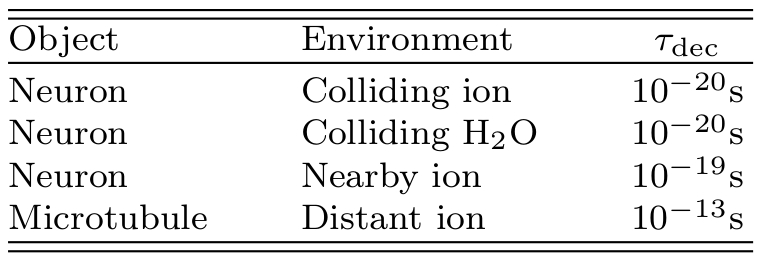
\includegraphics[scale=0.23]{graphics/decoherance_timescales.jpg}\,\cite{Tegmark_99}
				\end{column}}	
				\only<3>{\begin{column}{.45\textwidth}
					\centering
					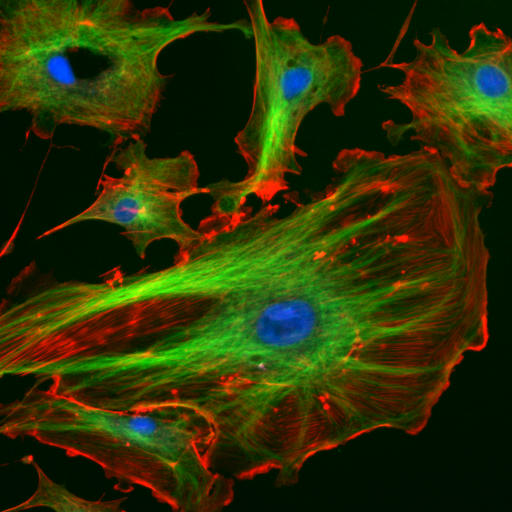
\includegraphics[scale=0.2]{graphics/FluorescentCells.jpg}\,\cite{microtubule}
				\end{column}
				\begin{column}{.55\textwidth}
					\centering
					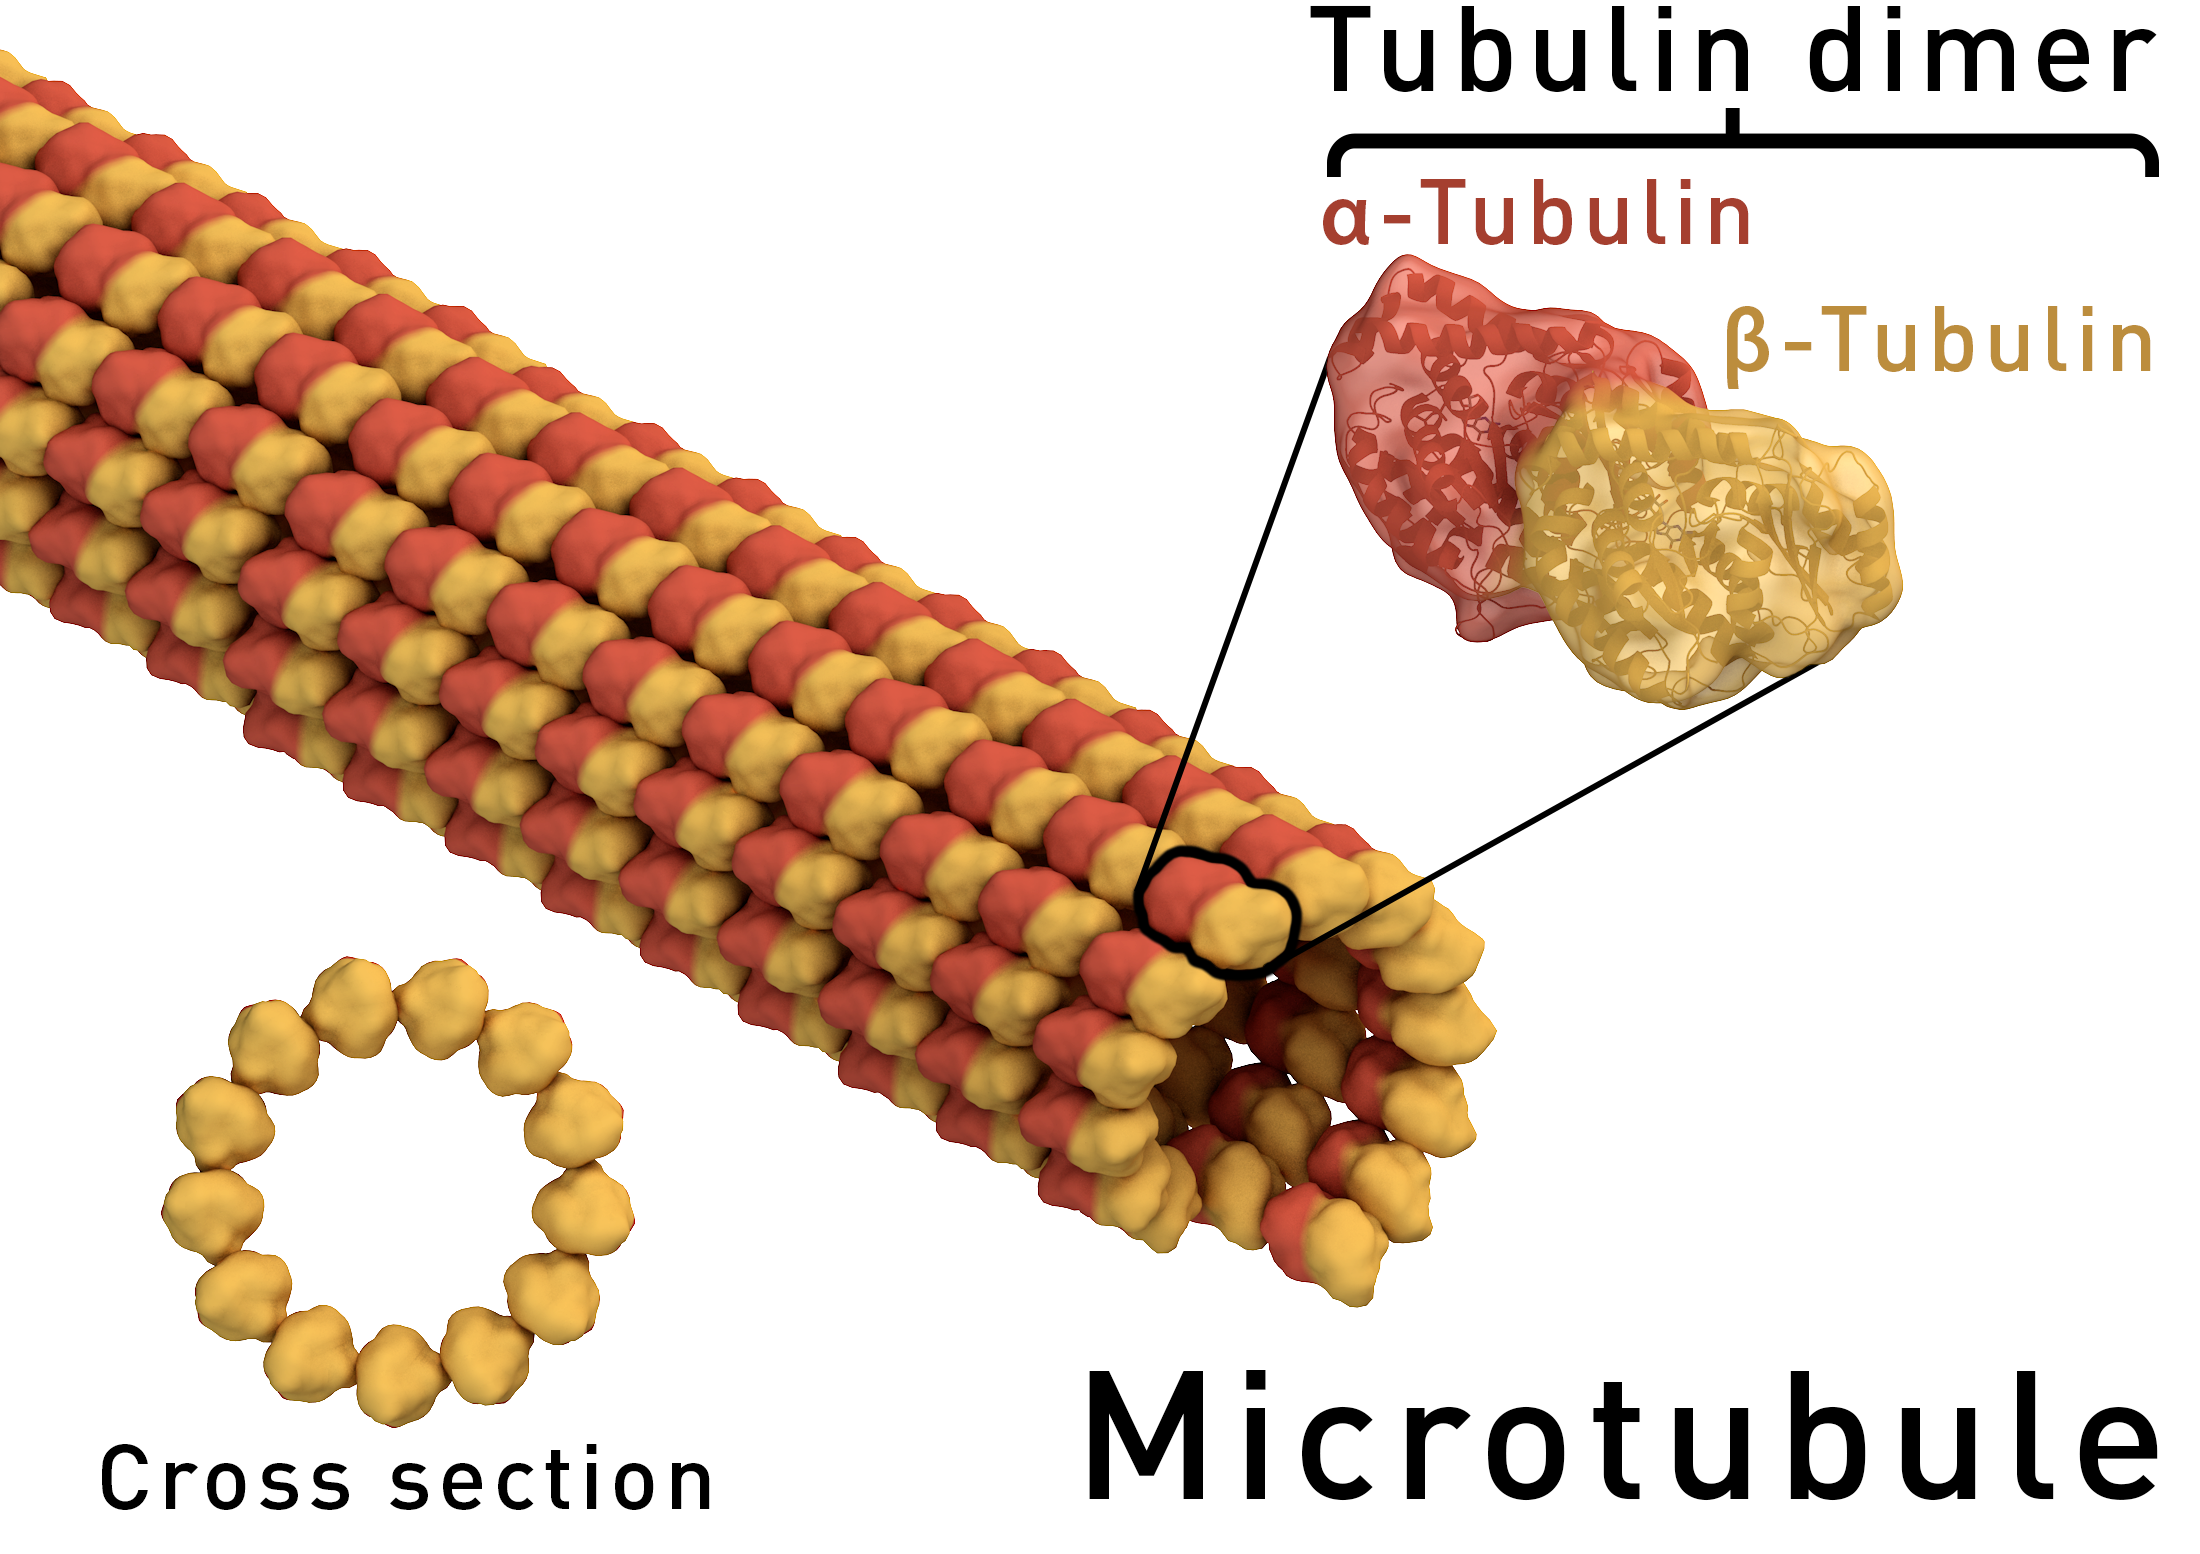
\includegraphics[scale=0.07]{graphics/Microtubule_structure.png}\,\cite{microtubule_structure}
			\end{column}}						
			\end{columns}
		 \alt<2>{\item{typische Dynamik-Zeitskalen sind $(\num{e-4} \text{ -- } 10^{0})\si{\second}$}
		 \begin{itemize}
		 	\item{Dekohärenz zerstört Superpositionen\\ schon bei der Entstehung}
		 	\item{Hirnprozesse als klassisch zu betrachten}
		 \end{itemize}}{}
		\end{itemize}}{}
\end{frame}